
\documentclass{article}

\usepackage[utf8]{inputenc}
%\usepackage{fontspec}
\usepackage{xeCJK}

\usepackage{multirow}
\usepackage{hyperref}
\usepackage{float}
\usepackage{array}
\usepackage{dirtytalk}
\usepackage{csquotes}
\usepackage{amsmath}
\usepackage{graphicx}
%
%
%\usepackage{xltxtra}

\title{Assessing Gender Bias in Machine Translation}
\author{Marcelo Prates \and Luis Lamb}

\begin{document}

\maketitle

\begin{abstract}
\end{abstract}

\section{Introduction}

Although the idea of automated translation can in principle be traced back to as long as the 17th century with René Descartes proposal of an \say{universal language} \cite{dascal1982universal}, machine translation has only existed as a technological field since the 1950s, with a pioneering memorandum by Warren Weaver \cite{weaver1955translation} discussing the possibility of employing digital computers to perform automated translation. The now famous Georgetown-IBM experiment followed not long after, providing the first experimental demonstration of the prospects of automating translation by the means of successfully converting more than sixty Russian sentences into English \cite{gordin2015scientific}. Early systems improved upon the results of the Georgetown-IBM experiment by exploiting Chomsky's theory of generative linguistics, and the field experienced a sense of optimism about the prospects of fully automating natural language translation. As is customary with artificial intelligence, the initial optimistic stage was followed by an extended period of strong disillusionment with the field, of which the catalyst was the influential ALPAC report \cite{hutchins1986machine}. Research was almost completely abandoned in the United States, making a shy re-entrance in the 1970s before the 1980s surge in statistical methods for machine translation \cite{koehn2009statistical}. Statistical and example-based machine translation have been on the rise ever since \cite{carl2003recent}, with highly successful applications such as Google Translate (recently ported to a neural translation technology \cite{wu2016google}) amounting to over $200$ million users daily \cite{bengio2015deep}.

In spite of the recent commercial success of automated translation tools (or perhaps stemming directly from it), machine translation has amounted a significant deal of criticism. Noted philosopher and founding father of generative linguistics Noam Chomsky has argued that the achievements of machine translation, while successes in a particular sense, are \emph{not successes in the sense that science has ever been interested in}: they merely provide effective ways, according to Chomsky, of approximating unanalyzed data. Chomsky argues that the faith of the MT community in statistical methods is absurd by analogy with a standard scientific field such as physics:

\begin{quotation}
I mean actually you could do physics this way, instead of studying things like balls rolling down frictionless planes, which can't happen in nature, if you took a ton of video tapes of what's happening outside my office window, let's say, you know, leaves flying and various things, and you did an extensive analysis of them, you would get some kind of prediction of what's likely to happen next, certainly way better than anybody in the physics department could do. Well that's a notion of success which is I think novel, I don't know of anything like it in the history of science.
\end{quotation}

Leading AI researcher and Google's Director of Research Peter Norvig responds to these arguments by suggesting that even standard physical theories such as the Newtonian model of gravitation are, in a sense, \emph{trained}:

\begin{quotation}
As another example, consider the Newtonian model of gravitational attraction, which says that the force between two objects of mass $m_1$ and $m_2$ a distance $r$ apart is given by

\begin{equation*}
F = G m_1 m_2 / r^2
\end{equation*}

where $G$ is the universal gravitational constant. This is a trained model because the gravitational constant G is determined by statistical inference over the results of a series of experiments that contain stochastic experimental error. It is also a deterministic (non-probabilistic) model because it states an exact functional relationship. I believe that Chomsky has no objection to this kind of statistical model. Rather, he seems to reserve his criticism for statistical models like Shannon's that have quadrillions of parameters, not just one or two.
\end{quotation}

Chomsky and Norvig's debate \cite{norvig2017chomsky} is a microcosmos of the two leading standpoints about the future of science in the face of increasingly sophisticated statistical models. Are we, as Chomsky seems to argue, jeopardizing science by relying on statistical tools to perform predictions instead of perfecting traditional science models, or are these tools, as Norvig argues, components of the scientific standard since its conception? Currently there are no satisfactory resolutions to this conundrum, but perhaps statistical models pose an even greater and more urgent threat to our society. On a 2014 article, Londa Schiebinger suggested that scientific research fails to take gender issues into account, arguing that the phenomenon of male defaults on new technologies such as Google Translate provides a window into this asymmetry \cite{schiebinger2014scientific}. Since then, recent worrisome results in machine learning have somewhat supported Schiebinger's view, and perhaps even partially confirmed some of Chomsky's fears. Not only Google photos' statistical image labeling algorithm has been found to classify dark-skinned people as gorillas \cite{garcia2016racist} and purportedly intelligent programs have been suggested to be negatively biased against black prisoners when predicting criminal behavior \cite{angwin2016machine} but the machine learning revolution has also indirectly revived heated debates about the controversial field of physiognomy, with proposals of AI systems capable of identifying the sexual orientation of an individual through its facial characteristics \cite{wang2017deep}. \emph{Machine bias}, the phenomenon by which trained statistical models unbeknownst to their creators become vessels of their own prejudices, is growing into a pressing concern for the modern times, and is an invitation for us to ask ourselves whether there are limits to our dependence on these techniques -- and more importantly, whether some of these limits have already been traversed.

With this in mind, we propose a quantitative analysis of the phenomenon of gender bias in machine translation. We believe this can be done by simply exploiting Google Translate to map sentences from a gender neutral language to English, as Figure \ref{fig:screenshot-gtranslate-hungarian} exemplifies.

\begin{figure}[h]
	\centering
	\fbox{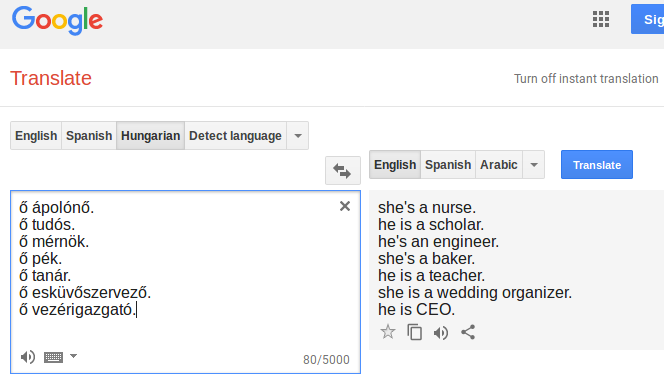
\includegraphics[width=\linewidth]{pictures/screenshot-gtranslate-hungarian}}
	\label{fig:screenshot-gtranslate-hungarian}
	\caption{Translating sentences from a gender neutral language such as Hungarian to English provides a glimpse into the phenomenon of gender bias in machine translation. This screenshot from Google Translate shows how occupations from traditionally male-dominated fields such as scholar, engineer and CEO are interpreted as male, while occupations such as nurse, baker and wedding organizer are interpreted as female.}
\end{figure}

\section{Motivation}

\section{Methods}

We believe that the phenomenon of gender bias in machine translation can be assessed by mapping sentences constructed in gender neutral languages to English by the means of an automated translation tool. Specifically, we can translate sentences such as the Hungarian \say{ő ápolónő}, where \say{ápolónő} translates to \say{nurse} and \say{ő} is a gender-neutral pronoun meaning either he, she or it, to English, yielding in this example the result \say{she's a nurse}. The same structure can be 

\begin{table}[H]
	\centering
	\begin{tabular}{|c|c|m{3cm}|c|}
	\hline
	Language Family & Language & Pronominal Gender System & Supported \\ \hline \hline
	\multirow{2}{*}{Austronesian} & Malay & No & Yes \\
	& Tagalog & No & \textbf{No} \\ \hline
	\multirow{3}{*}{Finno-Ugric} & Estonian & No & Yes \\
	& Finnish & No & Yes\\
	& Hungarian & No & Yes \\ \hline
	\multirow{4}{*}{Indo-European} & Armenian & No & Yes \\
	& Bengali & No & Yes \\
	& English & \textbf{Yes} & Yes \\
	& Persian & \textbf{Yes} & Yes \\ \hline
	\multirow{3}{*}{Indo-Aryan} & Maithili & No & \textbf{No} \\
	& Nepali & No & Yes \\
	& Oriya & No & \textbf{No} \\ \hline
	\multirow{10}{*}{} & Japanese & No & Yes \\
	& Korean & \textbf{Optional} & Yes \\
	& Turkish & No & Yes \\
	& Yoruba & No & Yes \\
	& Basque & No & Yes \\
	& Swahili & No & Yes \\
	& Chinese & \textbf{Optional} & Yes \\
	& Cantonese & No & \textbf{No} \\
	& Pipil & No & \textbf{No} \\
	& Quechuan & No & \textbf{No} \\ \hline
	\multirow{4}{*}{Constructed} & Esperanto & \textbf{Yes} & Yes \\
	& Ido & \textbf{Optional} & \textbf{No} \\
	& Lingua Franca Nova & No & \textbf{No} \\
	& Interlingua & No & \textbf{No} \\ \hline
	\end{tabular}
	\caption{Selected gender neutral languages obtained from the Wikipedia article \url{en.wikipedia.org/wiki/Gender_neutrality_in_genderless_languages}. Languages are grouped according to language families and classified according to whether they exhibit pronominal gender system. For the purposes of this work, we have decided to work only with languages lacking such a system, and as such Persian and Esperanto have been discarded. Because Tagalog, Maithili, Oriya, Cantonese, Pipil, Quechuan, Lingua Franca Nova and Interlingua lack support from Google Translate, these languages have also been ommitted from this work.}
\end{table}

\begin{table}[H]
	\centering
	\begin{tabular}{|c|c|}
	\hline
	Category 		& \# Occupations 	\\ \hline \hline
	Artistic 		& $102$ 			\\ \hline
	Computer 		& $19$ 				\\ \hline
	Corporate 		& $50$ 				\\ \hline
	Dance 			& $9$ 				\\ \hline
	Film/Television & $26$ 				\\ \hline
	Healthcare 		& $88$ 				\\ \hline
	Industrial 		& $26$ 				\\ \hline
	Science 		& $50$ 				\\ \hline
	Service 		& $10$ 				\\ \hline
	Theatre 		& $52$ 				\\ \hline
	Writing 		& $29$ 				\\ \hline
	\hline
	Total			& $461$				\\ \hline
	\end{tabular}
	\caption{Selected occupations obtained from the Wikipedia article \url{en.wikipedia.org/wiki/Lists_of_occupations}, grouped by category. We have selected a total of $453$ occupations from $11$ distinct groups (Artistic, Science, Service, etc.).}
\end{table}

\begin{table}[H]
	\centering
	\begin{tabular}{|c|c|}
	\hline
	Language 	& Sentence template \\ \hline \hline
	Malay		& dia adalah $\langle occupation \rangle$ \\ \hline
	Estonian	& ta on $\langle occupation \rangle$ \\ \hline
	Finnish		& hän on $\langle occupation \rangle$ \\ \hline
	Hungarian	& ő $\langle occupation \rangle$ \\ \hline
	Armenian	& նա $\langle occupation \rangle$ է \\ \hline
	Japanese	& は $\langle occupation \rangle$ です\\ \hline
	Turkish		& o bir $\langle occupation \rangle$ \\ \hline
	Yoruba		& o jẹ $\langle occupation \rangle$ \\ \hline
	Basque		& $\langle occupation \rangle$ da \\ \hline
	Swahili		& yeye ni $\langle occupation \rangle$ \\ \hline
	Chinese		& ta $\langle occupation \rangle$ \\ \hline
	\end{tabular}
	\caption{Templates used to infer gender biases in the translation to the English language.}
\end{table}

\section{Results}

\begin{table}[H]
	\centering
	\begin{tabular}{|c|c|c|c|c|c|}
	\hline
	Category & Female & Male & Neutral & Ratio & Total \\ \hline
	\hline
	Artistic        & 179    & 504  & 206     & 2.816 	& 918 \\ \hline
	Computer        & 7      & 125  & 39      & 17.857 	& 171 \\ \hline
	Corporate       & 36     & 340  & 74      & 9.444 	& 450 \\ \hline
	Dance           & 31     & 33   & 17      & 1.064 	& 81  \\ \hline
	Film-television & 54     & 125  & 55      & 2.315 	& 234 \\ \hline
	Healthcare      & 174    & 475  & 130     & 2.730 	& 792 \\ \hline
	Science         & 34     & 357  & 59      & 10.500 	& 450 \\ \hline
	Service         & 5      & 63   & 22      & 12.600 	& 90  \\ \hline
	Theatre         & 75     & 296  & 106     & 3.947 	& 477 \\ \hline
	Writing         & 41     & 148  & 72      & 3.610 	& 261 \\ \hline
	\hline
	Total           & 636    & 2466 & 780     & 3.877   &    \\ \hline
	\end{tabular}
	\label{tab:gender-by-category}
	\caption{Number of female, male and neutral pronominal genders per occupation category in the translated sentences. The corresponding sex ratios (\# Male / \# Female) show just how much male defaults are prominent in male dominated fields such as computer science, with up to $\approx 18$ occurrences of male pronouns for each of a female one.}
\end{table}

\begin{figure}[H]
	\centering
	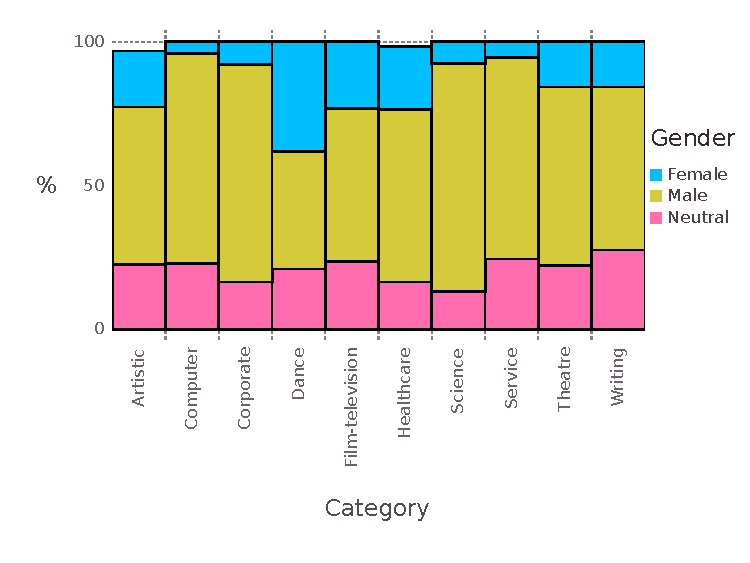
\includegraphics[width=\linewidth]{pictures/gender-by-category}
	\label{fig:gender-by-category}
	\caption{The distribution of pronominal genders in the translated sentences not only suggests a tendency towards male defaults but also reflects the structure of male dominated fields, with the proportion of male pronouns amounting to $73\%$ in computer related jobs and $76\%$ in corporate jobs respectively. Because Google Translate occasionally fails to translate a sentence, the bars for some categories fail to add up to $100\%$.}
\end{figure}

\begin{table}[H]
	\centering
	\begin{tabular}{|c|c|c|c|c|c|}
	\hline
	Language & Female & Male & Neutral & Ratio & Total \\ \hline
	\hline
	Malay     & 43     & 392  & 0       & 9.116 	& 436   \\ \hline
	Estonian  & 121    & 309  & 0       & 2.554 	& 436   \\ \hline
	Finnish   & 167    & 263  & 0       & 1.575 	& 436   \\ \hline
	Hungarian & 174    & 255  & 2       & 1.465 	& 436   \\ \hline
	Armenian  & 94     & 337  & 1       & 3.585 	& 436   \\ \hline
	Japanese  & 2      & 207  & 222     & 103.500   & 436   \\ \hline
	Turkish   & 19     & 368  & 44      & 19.368 	& 436   \\ \hline
	Yoruba    & 11     & 290  & 131     & 26.364 	& 436   \\ \hline
	Basque    & 5      & 45   & 380     & 9.000		& 436   \\ \hline
	Swahili   & 68     & 363  & 0       & 5.338 	& 436   \\ \hline
	Chinese   & 13     & 359  & 58      & 27.615 	& 436   \\ \hline
	\hline
	Total 	  & 717    & 3188 & 838     & 4.446     &   \\ \hline
	\end{tabular}
	\label{tab:gender-by-category}
	\caption{Number of female, male and neutral pronominal genders per language in the translated sentences. The corresponding sex ratios (\# Male / \# Female) show just how much male defaults are prominent in some languages such as Chinese, with almost 30 male pronouns for each female one.}
\end{table}

\begin{figure}[H]
	\centering
	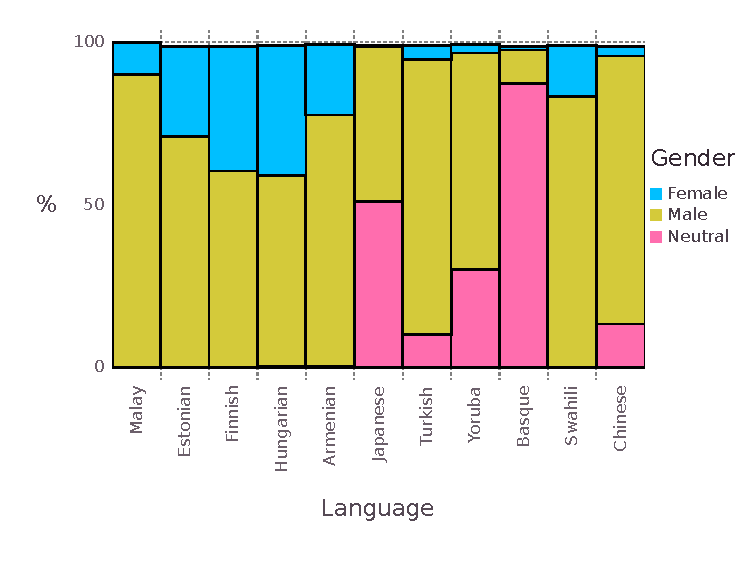
\includegraphics[width=\linewidth]{pictures/gender-by-language}
	\label{fig:gender-by-language}
	\caption{The distribution of pronominal genders per language also suggests a tendency towards male defaults, with female pronouns reaching as low as $0.46\%$ and $2.98\%$ for Japanese and Chinese respectively. Some languages such as Japanese (and particularly Basque) were observed to yield a high number of neutral pronouns, but that is the exception rather than the rule among the tested idioms. Once again not all bars add up to $100\%$ as Google Translate occasionally fails to translate sentences.}
\end{figure}

\begin{figure}[H]
	\centering
	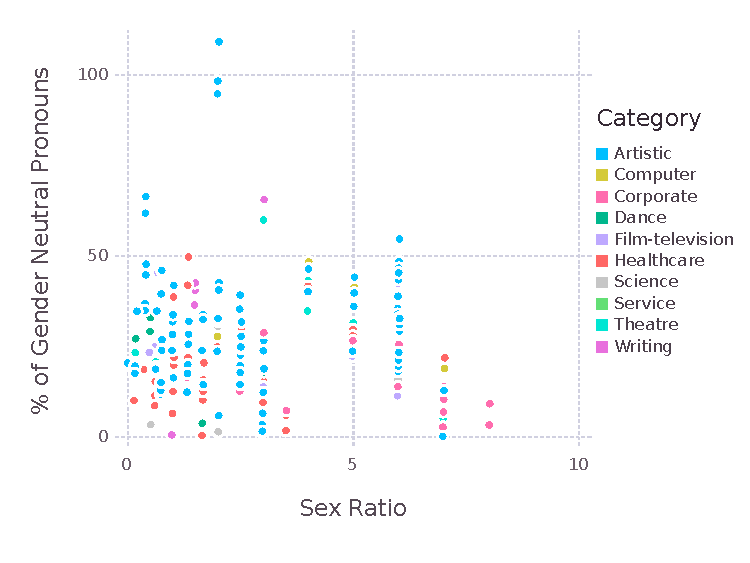
\includegraphics[width=\linewidth]{pictures/scatterplot-languages}
	\label{fig:scatterplot-languages}
	\caption{Scatter plot of translated sentences' statistics. Each point (color coded according to its category) corresponds to a single occupation, of which the sex ratio and the percentage of gender neutral pronouns are averaged over all tested languages (Malay, Estonian, Finnish, Hungarian, Armenian, Japanese, Turkish, Yoruba, Basque, Swahili and Chinese).}
\end{figure}

\section{Discussion}

\bibliographystyle{unsrt}
\bibliography{main}

\end{document}